\section{Descrição da estrutura}

A integração da sustentabilidade e da economia no desenvolvimento do projeto foi
um pilar fundamental para a tomada de decisões que nortearam a criação da
estrutura do nosso carrinho. Dessa forma, foram utilizados para compor a
estrutura, o material MDF para as laterais do carro, papelão para a parte
inferior e impressão 3D, com o filamento PLA (polímero termoplástico feito de
ácido lático feito a partir de matérias primas renováveis, como a mandioca,
milho, beterrada ou cana-de-açúcar) para a parte superior. Sendo assim, a
escolha por materiais recicláveis não apenas demonstra um compromisso da equipe
com a preservação ambiental, mas também oferece uma vantagem econômica ao
reduzir custos de produção. A impressão 3D, por sua vez, foi significativa na
personalização e na eficiência de fabricação, permitindo ajustes precisos que
beneficiam tanto a funcionalidade quanto a estética do produto final. Portanto,
ao incorporar esses princípios não só é cumprido os requisitos de
sustentabilidade e eficiência econômica, mas também se posicionam na vanguarda
da inovação, prontos para atender às necessidades de um futuro tecnológico em
constante mudança. No desenvolvimento do projeto, foi adotado um design
minimalista que favorecesse a utilização dos materiais previstos. As dimensões
foram especificadas com margens levemente superiores ao necessário, permitindo a
inclusão de novos componentes ou o rearranjo dos elementos atuais sem exigir um
redimensionamento completo da estrutura. Uma decisão crucial no projeto foi a
implementação de \textit{slots} na base, permitindo que a parte superior fosse
encaixada e removida facilmente, facilitando o acesso e manutenção dos circuitos
internos. Para a fixação das laterais de MDF com a parte superior em impressão
3D, foi utilizado adesivo instantâneo.

A seguir, são apresentadas as dimensões e características da estrutura do robô.

\begin{figure}[htb]
  \caption{\label{fig:structure-down} Visão inferior do robô}

  \begin{center}
    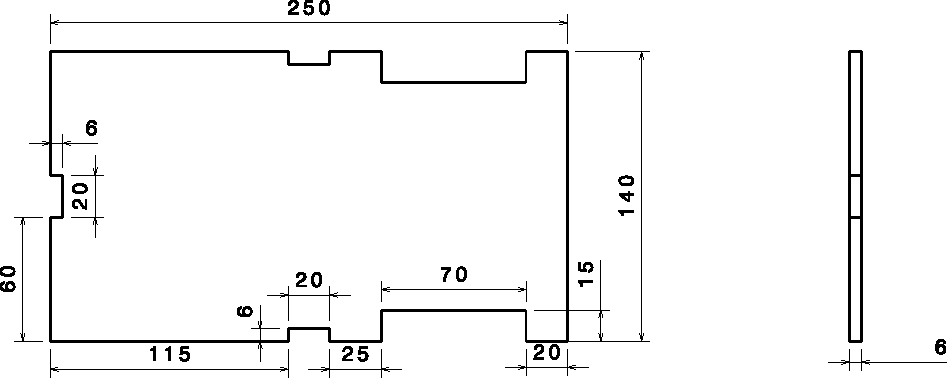
\includegraphics[scale=0.525,page=1]{../img/structure.pdf}
  \end{center}

  \legend{Fonte: Elaborado pelos autores.}
\end{figure}

\begin{figure}[htb]
  \caption{\label{fig:structure-side} Visão lateral do robô}

  \begin{center}
    \includegraphics[scale=0.525,page=2]{../img/structure.pdf}
  \end{center}

  \legend{Fonte: Elaborado pelos autores.}
\end{figure}

\begin{figure}[htb]
  \caption{\label{fig:structure-back} Visão traseira do robô}

  \begin{center}
    \includegraphics[scale=0.525,page=3]{../img/structure.pdf}
  \end{center}

  \legend{Fonte: Elaborado pelos autores.}
\end{figure}

\begin{figure}[htb]
  \caption{\label{fig:structure-front} Visão frontal do robô}

  \begin{center}
    \includegraphics[scale=0.525,page=4]{../img/structure.pdf}
  \end{center}

  \legend{Fonte: Elaborado pelos autores.}
\end{figure}

\begin{figure}[htb]
  \caption{\label{fig:structure-up} Visão superior do robô}

  \begin{center}
    \includegraphics[scale=0.525,page=5]{../img/structure.pdf}
  \end{center}

  \legend{Fonte: Elaborado pelos autores.}
\end{figure}

\begin{figure}[htb]
  \caption{\label{fig:structure-iso} Visão isométrica do robô}

  \begin{center}
    \includegraphics[scale=0.525,page=6]{../img/structure.pdf}
  \end{center}

  \legend{Fonte: Elaborado pelos autores.}
\end{figure}

%
% Comando para pular todo o conteúdo a seguir para a próxima página, para
% evitar que a figura fique no final da próxima seção.
%
\newpage
